\chapter{Simulation}

\section{Introduction}
How we said in the previous chapter we built the model inside the framework \textbf{OMNeT++ v5}. The definition of network \textit{(CellularNetwork.ned)} and their components can be found in the directory \textit{RRCellNet/src}. We decided to analyze it when 10 \texttt{Mobile Stations} are connected to the \texttt{Antenna}. In order to simplify the model we represented the network with a \textit{Star Topology}. \texttt{Mobile Stations} receive packets through unicast channel \texttt{without transmission delay}.

We recall that \texttt{Web Servers} are sources of packets addressed to \texttt{Mobile Stations}. In order to have true random and independent arrivals to \texttt{Antenna} we need a 10 RNG, one for each \texttt{Web Server}. We also need RNG to generate packets with random size so others 10 RNG are neeeded. We need also a RNG for each \texttt{Mobile Station} in order to generate random CQIs at each timeslot. Overall the model requires 30 RNGs each of them initialized with a different seed in order to have independent pseudo-random variables. The seed-set is changed at every repetition to have different independent experiments. At the end of all repetions the results are aggregated by computing the mean and 95\% confidence interval. 

Let's consider for example the mean throughput for a rate \(\lambda^{*}\). By running each repetition we get the values \(X_{1},X_{2},\ldots X_{10}\). \(X_{i}\) is a random variable which represents the mean throughput for the repetition \(i\). By the CLT theorem we can say that \(X_{i}\) is a normal RV since it is obtained by summing up a huge number of \textit{slotted throughput}. We can estimate the mean \(\bar{X}\) and a 95\% confidence interval by using the \textit{Student's t distribution} because \(X_{i}\) are normal RV. 

\begin{align}
	\bar{X} &= \frac{X_{1}+X_{2}+\ldots+X_{10}}{10} \qquad S^{2} = \frac{1}{9}\sum_{i=1}^{10}(X_{i} - \bar{X})^{2} \\
	CI_{0.95} &= \left[\bar{X} - \frac{S}{\sqrt10}t_{0.025,9}, \: \bar{X} + \frac{S}{\sqrt10}t_{0.025,9}\right]
\end{align}

Similar consideration can be done for others quanties wich we will analyze during simulations. Once we have computed the mean \(\bar{X}\) and its confidence interval we can do a box plot for that quantity at varying workload \(\lambda\) as required by specifications. Data are exported from simulation to csv files through a bash script \textit{exportdata.sh} and plots are done through an R script \textit{analyze\_csv.r}. These script are both included in the directory \textit{RRCellNet/simulations}.

All parameters for simulations are summarized here and can be found in the file \textit{RRCellNet/simulations/omnetpp.ini}. We will use them in the following chapters unless otherwise specified.
\begin{itemize}
\item \textbf{Number of resource block}, \(\#RB = 25\)
\item \textbf{Number of users}, \(n = 10\)
\item \textbf{Number of RNG}, \(\#RNG = 30\)
\item \textbf{Max RB size}, \(RBsize\textsubscript{max} = 93\)
\item \textbf{Max packet size}, \(packetsize\textsubscript{max} = 75\)
\item \textbf{Timeslot period}, \(T\textsubscript{slot} = 1\textnormal{ms}\)
\item \textbf{Number of repetions}, \(\#REP = 10\)
\item \textbf{Simulation time}, \(ST = 60 \textnormal{s}\)
\item \textbf{Warmup period}, \(WP = 0.3 \textnormal{s}\)
\end{itemize}

\section{Warm-Up Period Estimation}
In the previous section we saw that the warm-up time is 0.3s, but we haven't specified yet how that value comes out.

In this section we will illustrate how we have estimated the length of the warm-up period. We followed this approach: for each scenario and for each user we plotted the graph of the throughput and the response time and then for each repetition we applied the sliding moving average and then we computed the sample mean of the latter in order to see how many time it was required to converge around that value.
We chosen the worst case among all of them, which graph is the following:

\begin{figure}[H]
  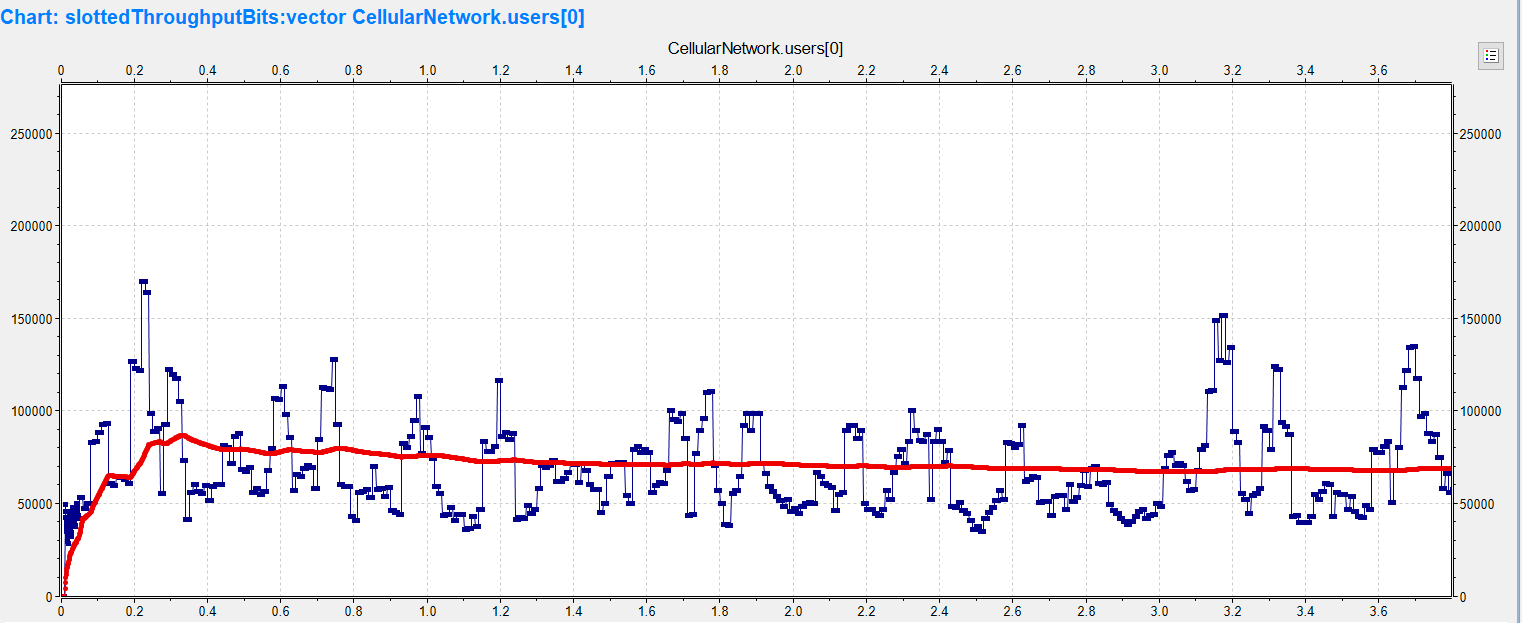
\includegraphics[width=1\textwidth]{images/binomial_user0_rate9_6_rep9}
  \caption{Worst Case for the Warm-Up period estimation}
  \label{fig:warm_up time}
\end{figure}

So we saw that in the worst case the graph converged to the sample mean after \textbf{0.5s} and we chosen that value as \textbf{warm-up time}. 